
\section{Evaluation}
\label{sec:results}

We now present an evaluation of \tool. In \xref{sub:accuracy}, we evaluate
\tool's effectiveness by measuring the quality of patches and related
instrumentation required. We also measure how the several optimizations
described in \xref{subsec:optimizations} affect the patches generated by \tool.
In \xref{sub:overhead}, we measure the relative performance and resource
penalties incurred with \tool. In \xref{sub:casestudies}, we describe our
experiences with $x$ major bugs from our data set.

\myparagraph{Data Set} We mined bug repositories of several \java-based
applications from hugely popular product suites including Apache, Eclipse,
JBoss, etc., and selected $30$ bugs, majority of them being rated either major,
critical or blocking. These bugs involved usage of $64+$ different APIs from
\java's \code{String}, \code{StringBuffer}, \code{StringBuilder}, and Apache
\code{StringUtils} and Google Guava \code{StringUtils} classes.

% \begin{mylist}
% 
% \item \textbf{Popularity}: How much it is used among the developers and
% industries,
% \item \textbf{Severity} : We consider major, critical and blocker priority bugs
% only considering the facts at the bug affects dependent applications and other
% libraries severely.
% \item \textbf{Age and state} : We consider latest bugs which were reported in
% the last 5 years.
% We also consider such bugs which still remains un-fixed.
% 
% \end{mylist}

\myparagraph{Experimental Setup} All our experiments were performed on a laptop
with $2.9$ GHz dual core Intel i$5$ CPU, and $8$ GB of RAM, and running
Microsoft Windows $8.1$. We used JDK v$1.7$ running with $2$ GB of allocated
heap space. All bug reproduction was done on Eclipse Juno IDE. We used \soot\
v$2.5.0$ for bytecode analysis and instrumentation, and \soot\ \infoflow\ v$xxx$
for static taint analysis.
% We have also used \java\ decompiler JD v0.7.

% 
% equipped with a dual core Intel i5
% 2.3-2.9 GHz processor, 8 GB or RAM, Microsoft Windows 8.1 operating system, JDK
% version 1.7-45 with 2 GB of allocated heap space. All the bug reproduction was
% done on
% Eclipse Juno IDE. For static analysis and instrumentation we have used \soot\
% version 2.5.0 and \soot\ \infoflow\ for static taint analysis. We have also used
% java decompiler JD version 0.7.0.1. 

\subsection{Accuracy}
\label{sub:accuracy}

We evaluate the precision of the patch and the effectiveness of \tool\ based on
several metrics as described below.

% We have conducted the evaluation based on the matrices which empirically
% measures the precision and the performance of the developed tool. We measures
% the precession in terms of the quality of the patch and some other criteria
% listed bellow and the performance based on the time taken and the memory
% footprint.

\begin{mylist}

\item \textbf{Effectiveness of the patch}: Precision and effectiveness of a
patch is governed by the similarity between a \tool\ generated patch and the
developer's fix for the same bug. We define \textbf{Patch Quality Index (PQI)}
as a measure of the effectiveness of the patch.
$$PQI = \frac{\#~Constraints_{Similar}}{\#~Constraints_{Developer}} *
\frac{\#~LOC_{\tool}}{\#~LOC_{Developer}} *
\frac{Output_{\tool}}{Output_{Developer}}$$

Specifically, PQI compares the similarities in constraints and source line of
code in \tool's patch against the developer's version, as well as the actual
output generated from both the patches, thereby considering both the logic and
the technique to construct an effective patch. A higher value of PQI is
preferred.

% is the This matrix is for
% the qualitative analysis of our auto generated patches. By this measurement we
% have not only ensure the effectiveness of the patch but also look at the
% similarity of logic an patch construction with the developers' one.After the
% patching we compared both the auto-generated patch code with the developer's
% patching code we found in the bug repositories. In the case the bug is still
% un-fixed we looked for the comments and discussion in the panel and collects
% the information about the potential patch. At the first step, we visually
% compared the patches to see how much they are similar and dissimilar with the
% developers' patch.

Determining PQI is a three step process. First, we visually compare \tool's
patch with the developer's version and count the exact similar constraints
observed in both patches to determine the closeness in terms of the set of
constraints. Second, we
disassembled the developer's patch and compared the count of bytecodes generated
using \tool's patch. Lastly, we observed the actual output of using the \tool\
patched class files against the developer provided patch in a later version of
the same library. In case the output is primitive or strings, an exact
match is considered successful, else we iterate over the properties of the
complex object to determine similarities.

% In case the results were either primitive or string type, we
% compared the output. In case the output is some complex object we compare
% the properties of them.

% Apart
% from the test cases to reproduce the bug, we also ran couple of good test case
% to make sure that the patch is not behaving any other way. Based on this
% experiment we made a metric named \textbf{Patch Quality Index (PQI)} which
% can contains three values, high, medium and low where we consider high PSI being
% a good close quality patch.


%% subsumed in PQI

% \item \textbf{Auto-generated patch size and the develops' patch size} : Apart
% from the qualitative analysis we have measured quantitative aspect of the
% Auto-generated patches and compared their sizes with the developers' one.
% Quantitative measurement comes to picture only when we are satisfied with the
% qualitative measurement. We came up with a metric called \textbf{Patch Size
% Index (PSI)}. In case our patch is qualitatively satisfactory and the size is
% less than the developer one the we assign PSI as high. In case the size varies
% in $\pm5\%$ we assign PSI as medium. If our patch is more than $5\%$ bigger than
% the develops' one then PSI is assigned to low.

\item \textbf{Already handled exceptions}: \tool\ analyzes the call graph to
determine if a potential runtime exception throwing statement is handled higher
up in the call chain or in the same method. In such cases \tool\ must abort the
patching effort considering that the exception is caught with exact exception
type or its base type, else it will disrupt the normal control flow of the
program. We measure the extent of this optimization, which prevents disruption
of the control flow using the \textbf{Program Flow Consistency Index (PFCI)}
which is calculated as $$PFCI = \frac{Patch_{HE}}{Stmt_{HE}}$$ where
$Patch_{HE}$ = \# patches placed in already handled exceptions, and
$Stmt_{HE}$ =  \# statements in the program which are already handled. We
observe that $0 \le PFCI \le 1$, and a lower value of $PFCI$ is desirable.

\item \textbf{Cascaded exception}: A cascaded exception arises if
the auto-generated patch creates objects that when used as inputs to other
\java\ APIs result in further exceptions.
% patched objects
% are used as a input
% to other methods and violates the specification there.
\tool\ is prone to cascading exceptions because of the limitation of its
intra-procedural analysis and a simple, yet effective, constraint evaluation
mechanism. However, \tool's constraint solver is pluggable and a more
sophisticated third party solvers can easily be integrated.
% This is the limitation
% in our technique in the some complicated cases where it requires develops' 
% attention. The limitation is due to the fact that the analysis for the
% repairing 
% technique is a intra-procedural analysis and the constraint evaluation method is
% very simple. For the constraint evaluation part, the solver is pluggable, we can
% easily replace it with a third party solver.
Specifically, cascaded exceptions may arise if the patch generates \code{String}
objects that represent a malformed string. Further, if we keep the optimization
in \xref{subsubsec:minimizePatchInstrumentation}, then cascaded failures may
occur even for subsequent \code{String} APIs handling the malformed
string following the point of patching. If the optimization is turned
off, \tool\ will automatically patch all relevant \code{String} APIs and thus
handle all cascaded failures involving malformed \code{String} objects.
% 
% Cascaded exception can be noticed
% when the string object we are patching is generation some specific URI or driver
% string which would be used to load or configure something. In such scenario, the
% patch may produce some malformed string. In case there is a cascaded exception 
% in string object, our analysis will take care of it, other wise it would abort. 
\end{mylist}

% \subsection{Experimental Results}
% \label{subsec:experimentalResults}

\begin{table*}[t]
% \setlength{\tabcolsep}{3pt}
\centering
\scriptsize
\begin{tabular}{|l|l|l|l|c|r|r|r|r|c|}

\hline

\multicolumn{1}{|c|}{\textbf{API}} &
\multicolumn{1}{c|}{\textbf{BugID}} &
\multicolumn{1}{c|}{\textbf{Priority}} &
\multicolumn{1}{c|}{\textbf{$PQI$}} &
\multicolumn{1}{c|}{\textbf{$PFCI$}} &
\multicolumn{1}{c|}{\textbf{$\mathcal{N}_{Unit}$}} &
\multicolumn{1}{c|}{\textbf{$\mathcal{IC}_{NO}$}} & %instrumentation with
%optimization
\multicolumn{1}{c|}{\textbf{$\mathcal{IC}_{WO}$}} & %instrumentation without
%optimization
\multicolumn{1}{c|}{\textbf{$\mathcal{N}_{CG}$}} &
%\multicolumn{1}{c|}{\textbf{$\mathcal{PF}_{CA}$}} & %profile for constraint
%\multicolumn{1}{c|}{\textbf{$\mathcal{PF}_{TA}$}} & %profile for taint analysis
%\multicolumn{1}{c|}{\textbf{$\mathcal{PF}_{CG}$}} & %profile for call graph
%\multicolumn{1}{c|}{\textbf{$\mathcal{PF}_{IN}$}} & %profile for
% instrumentation
\multicolumn{1}{c|}{\textbf{$\mathcal{RS}_{CE}$}}\\ % cascaded exception

\hline
%% 1.02238806
\code{Aries} & \cite{ARIES1204} & Major & $ 1.02$ & $0$ &$129$ &$42$& $5$
&$3.5K$ 
%$3.1/10$ & $0.6/31$ & $12.8/146$ &$2.3/142$ 
& $\checkmark$ \\
%% 0.791666667
\code{Commons CLI1.x} & \cite{CLI193} & Critical & $0.79
 $ & $0$ & $53$ & $19$& $19$
& $3.2K$
%& $2.8/5$ & $0.5/30$ & $11.6/149$ & $1.9/133$ 
& $\checkmark$ \\
%% 0.5
\code{Commons CLI2.x} & \cite{CLI46} & Major & $0.50
 $ & $1$ & $21$ & $13$
&$2$ & $3.2K$ 
%& $2.8/5$ & $0.6/32$ & $12/212$ & $2/131$ 
& $\times$ \\
%% 0.992753623
\code{Commons Compress} & \cite{COMPRESS26} & Blocker & $0.99
 $ & $0$ &
$134$& $46$& $4$ & $4K$ 
%$2.7/5$ & $0.5/30$ & $11.5/209$ & $1.8/130$ 
&$\checkmark$\\
%% 1.015873016
\code{Commons IO} & \cite{IO179} & Major & $ 1.01
$ & $0$ & $125$ & $76$ &
$1$& $3.3K$  
%$3/11$ & $0.5/33$ & $12/209$ & $2/141$ 
& $\checkmark$\\
%% 0.983870968
\code{Commons Lang} & \cite{LANG457} & Major & $0.98
 $ & $0$ & $240$ & $168$&
$8$ & $5.1K$  
%$3/19$ & $0.57/30$ & $16.5/209$ & $2.8/158$ 
& $\checkmark$ \\
%% 1
\code{Commons Math} & \cite{MATH198} & Major & $1.00
 $ & $0$ & $300$ & $36$
&$2$ & $3.4K$  
%$3/20$ & $0.5/30$ & $11.9/209$ & $2.9/152$ 
& $\checkmark$ \\
%% 1.066666667
\code{Commons Net} & \cite{NET442} & Major & $ 1.07
$ & $0$ & $14$ & $6$ &
$1$& $3.3K$  
%$2.8/6$ & $0.5/33$ & $11.4/212$ & $1.9/132$ 
& $\checkmark$ \\
%% 1
\code{Commons VFS} & \cite{VFS338} & Major & $1.00
 $ & $0$ & $37$ & $20$ & $2$
&$4.5K$ 
%$3.7/13$ & $1.4/7$ & $46.1/151$ & $3.1/143$ 
& $\checkmark$ \\
%% 0.956521739
\code{Derby} & \cite{DERBY4748} & Major & $0.96
 $ & $0$ &$40$ & $47$ & $6$ &
$4.4K$  
%$3.3/15$ & $0.5/31$ & $19.9/208$ & $2.7/146$ 
& $\checkmark$ \\

%% 0.942857143
\code{DUMMY 4 compilation} & \cite{DUMMY} & Major & $0.94$ & $0$ & $33$ & $13$
& $2$& $3.3K$
%& $2.7/8$ & $0.5/33$ & $13.5/213$ & $2.2/131$
& $\checkmark$ \\

%% 0.519607843
\code{Eclipse AJ Weaver} & \cite{EclipseBug432874} & Major & $ 0.52
$
&$0$ & $50$ & $4$ & $1$ & $20.6K$ 
%& $3.1/18$ & $0.6/34$ & $41.2/212$ &$1.6/142$
& $\times$ \\
%% 1.025
\code{Eclipse AJ} & \cite{EclipseBug333066} & Major & $1.03
 $ & $0$
&$39$ & $6$ & $1$ & $25K$  
%$3.8/24$ & $0.5/34$ & $43.6/214$ & $1.6/156$
&$\checkmark$ \\
%% 0.960
\code{FlexDK 3.4} &\cite{SDK14417} & Minor  & $0.96
 $ & $0$ & $600$ & $207$ &
$25$ & $6.3K$  
%$4.8/40$ & $0.4/31$ & $12.9/209$ & $2.6/189$ 
& $\checkmark$ \\
%% 0.956521739
\code{Hama 0.2.0} &\cite{HAMA212}  & Critical  & $1.38
 $ & $0$ & $35$ & $28$
& $5$ & $3.7K$  
%$2.6/5$ & $0.5/33$ & $14.4/210$ & $3.1/134$ 
& $\checkmark$ \\
%% 1.015873016
\code{HBase 0.92.0} &\cite{HBASE4481}  & Critical  & $ 1.01
$ & $0$ & $61$ &
$13$ & $2$ & $4.8K$  
%$3.2/15$ & $1.4/11$ & $18.9/212$ & $3.1/144$
& $\checkmark$\\
%% 1.015873016
\code{Hive} &\cite{HIVE6986} & Trivial & $1.01
 $ & $0$ & $23$ & $8$ & $1$
&$4.4K$  
%$3.4/12$ & $1.5/11$ & $20/121$ & $1.6/143$ 
& $\checkmark$ \\
%% 0.956521739
\code{HttpClient} &\cite{HTTPCLIENT150} & Major & $1.13

 $ & $0$ & $14$ & $6$&
$1$ & $3.3K$  
%$2.8/6$ & $0.5/33$ & $12.3/212$ & $2.7/131$ 
& $\checkmark$ \\
%% 1.133333333
\code{jUDDI} & \cite{JUDDI292} & Major & $ 1.13
$ & $0$ & $70$ & $10$ & $2$
&$3.2K$ 
%$3.1/11$ & $0.5/34$ & $13.6/209$ & $2.9/138$ 
& $ \checkmark$ \\
%% 0.972222222
\code{Log4j} & \cite{ApacheLog4jBug} & Major & $ 0.97

$ & $0$ & $17$ & $6$
&$1$ & $3.2K$  
%$2.8/4$ & $0.5/32$ & $13/212$ & $2.5/131$ 
& $\checkmark$ \\
%% 1
\code{MyFaces Core} & \cite{MYFACES416} & Major & $1.00
 $ & $0$ & $50$ & $4$&
$2$ & $4.5K$  
%$3.8/4$ & $0.5/30$ & $17/218$ & $1.6/130$ 
& $\checkmark$ \\
%% 0.980769231
\code{Nutch} & \cite{NUTCH1547} & Major & $0.98

 $ & $0$ & $90$ & $8$&
$1$ & $4.5K$  
%$3.2/15$ & $1.2/30$ & $32.9/215$ & $3.9/147$ 
& $\checkmark$ \\
%% 1.010989011
\code{Ofbiz} & \cite{OFBIZ4237} & Minor & $1.01

 $ & $1$ & $28$ & $6$ &$1$ &
$4.4K$  
%$3.1/15$ & $1.3/14$ & $18.9/215$ & $2.8/149$ 
& $\checkmark$ \\
%% 1.137931034
\code{PDFBox} & \cite{PDFBOX467} & Major & $ 1.14

$ & $0$ & $23$ & $8$& $1$ &
$4.4K$  
%$3.3/12$ & $1.5/1$ & $20/212$ & $2.6/143$ 
& $\checkmark$ \\

%\code{Servicemix-soap} & \cite{SMXCOMP156} & Major & High & $0$ & $$ & $$&
%$$ & $$ & $$ & $$ & $$ & $$ & $\checkmark$ \\
%% 1
\code{Sling Eclipse IDE} & \cite{SLING3095} & Major & $ 1.00
$ & $0$ & $58$
&$39$ & $6$ & $4.5K$  
%$3/14$ & $0.5/34$ & $21.3/208$ & $3.5/147$ 
& $\checkmark$\\
%% 0.96875
\code{SOAP} & \cite{SOAP130} & Major & $0.97
 $ & $0$ & $165$ & $32$ & $5$
&$5K$  
%$3.4/19$ & $0.6/30$ & $14/209$ & $2.3/148$ 
& $\checkmark$ \\
%% 0.976470588
\code{SOLR 1.2} & \cite{SOLR331} & Major & $0.98
 $ & $0$ & $200$ & $25$ &
$4$& $11K$  
%$4.4/21$ & $0.6/32$ & $24/219$ & $2.7/139$ 
& $\checkmark$ \\
%% 1.024509804
\code{Struts2} & \cite{WW650} & Major & $1.03
 $ & $0$ & $80$ & $25$ & $2$
&$16K$  
%$3/14$ & $0.5/32$ & $25.9/210$ & $1.3/140$ 
& $\checkmark$ \\
%% 0.975609756
\code{Tapestry 5} & \cite{TAP51770} & Major & $0.98
 $ & $0$ & $71$ & $31$
&$5$ & $6.2K$  
%$2.9/10$ & $0.5/34$ & $2.4/211$ & $1.9/136$ 
& $\checkmark$ \\
%% 0.960526316
\code{Wicket} & \cite{WICKET4387} & Major & $0.96
 $ & $0$ & $68$ & $16$ &
$1$& $70K$  
%$3/14$ & $0.5/32$ & $52.4/210$ & $1.4/142$ 
& $\checkmark$ \\
%% 1.028985507
\code{XalanJ2} & \cite{XALANJ836} & Major & $ 1.03

$ & $0$ & $33$ & $13$ &
$2$& $3.3K$  
%$2.7/8$ & $0.5/33$ & $13.5/213$ & $2.2/131$ 
& $\checkmark$ \\

\hline

\end{tabular}

\caption*{
\scriptsize
\centering
\setlength{\tabcolsep}{3pt}
\begin{tabular}{ll|ll|ll|ll}
$PQI$ & Program Quality Index & $PFCI$ & Program Flow Consistency Index &
$\mathcal{N}_{Unit}$ & Total \#\code{Units} analyzed & \\
$\mathcal{IC}_{NO}$ & Instrumentation without optimization & $\mathcal{IC}_{WO}$
& Instrumentation with optimization & $\mathcal{N}_{CG}$ & Size of the call
graph & $\mathcal{RS}_{CE}$ & If cascaded exception exists\\
\end{tabular}
}
\caption{Experimental results.}
\label{tab:results}
\end{table*}

% \begin{table}[t]
% \centering
% \scriptsize
% \begin{tabular}{|l|l|}
% \hline
% \multicolumn{1}{|c|}{\textbf{Notation}} &
% \multicolumn{1}{c|}{\textbf{Meaning}} \\
% 
% \hline
% API & Analyzed library\\
% BugID & Unique ID in bug repository\\
% Priority & Severity of bug \\
% $PQI$ & Program Quality Index\\
% $PSI$ & Program Size Index\\
% $PFCI$ & Program Flow Consistency Index\\
% $\mathcal{N}_{Unit}$ & Total \#\code{Units} analyzed\\
% $\mathcal{IC}_{NO}$ & Instrumentation without optimization\\
% $\mathcal{IC}_{WO}$ & Instrumentation with optimization\\
% $\mathcal{N}_{CG}$ & Size of the call graph\\
% %$\mathcal{PF}_{CA}$ & Profiling data of constraint analysis(sec/MB)\\
% %$\mathcal{PF}_{TA}$ & Profiling data of taint analysis(sec/MB)\\
% %$\mathcal{PF}_{CG}$ & Profiling data of call graph(sec/MB)\\
% %$\mathcal{PF}_{IN}$ & Profiling data of instrumentation phase(sec/MB)\\
% $\mathcal{RS}_{CE}$ & If cascaded exception exists\\
% 
% \hline
% \end{tabular}
% 
% \caption{Notations used in Table~\ref{tab:results}}
% \label{tab:Notation}
% \end{table}

\todo{Describe in detail the results.}

Table~\ref{tab:results} lists $30$ real-world and $5$ synthetic bugs that we
have patched using \tool, along with the several accuracy metrics described
above. We observe that PQI for \tool\ generated patches is high for most of
the bugs, which indicates the effectiveness of the patches. However, we also
note that for $x$ bugs the PQI was low. This is because \todo{Add more details
later}.

24 out of 30 patches were within 7\% of the developer's fix, while only 4 were 

However, there were instances where the concerned bug
was still unpatched. In such cases, we looked for the potential or suggested
patches in comments and discussion forums for the specific product.


\subsection{Overhead}
\label{sub:overhead}

We measure the overhead of \tool\ using different parameters as identified
below.

\begin{mylist}

 \item \textbf{Execution overhead}: We determine the execution overhead of the
patched class files and compare it with the developer's patch to demonstrate
the execution overhead of patches generated by \tool. Figure~\ref{fig:perf:exec}
plots the overhead for all the benchmarks studied in Table~\ref{tab:results}. We
note that the execution overhead of \tool's patches is less than $x\mu$s, which
is imperceptible at human response times.

 \item \textbf{Constraint set}: \tool\ performs an exhaustive multi-pass
analysis to gather and evaluate the set of constraints for generating patches. A
higher number of constraints and their complexity increases the duration of
\tool's analysis. Figure~\ref{fig:perf:constraints} compares the time required
for analysis with an increasing number of constraints for the benchmarks used in
our data set.

 \item \textbf{Number of \code{String} objects}: \tool\ performs exhaustive
optimizations to limit the static and dynamic instrumentations at points of
interest. Thus, \tool's performance is also dependent on the number of
\code{String} objects. Figure~\ref{fig:perf:strings} plots the trend in analysis
time as a function of the \code{String} objects generated for our benchmarks.
We observer that \todo{Add details later.}.

 \item \textbf{Call graph}: The size of the call graph directly governs the time
and memory consumption for \tool. Figure~\ref{fig:perf:callgraph} shows the
results for the bugs analyzed in our data set. We observe that for the
\code{Wicket} benchmark, \tool\ generates a call graph of $\sim$$70K$ nodes, and
requires $52.4$s and $210$MB memory for complete end-to-end analysis.

\end{mylist}

%%%%Table for the taint analysis stats
\begin{table}[t]
\centering
\scriptsize
\begin{tabular}{|l|c|c|c|}
\hline
\multicolumn{1}{|c|}{\textbf{Application}} &
\multicolumn{1}{c|}{\textbf{KLOC}} & 
\multicolumn{1}{c|}{\textbf{Statements}} & 
\multicolumn{1}{c|}{\textbf{Flagged by taint analysis}}\\

\hline
\code{checkstyle4j}& $58K$ & $66K$ & $28$\\
\code{Jazzy}& $4.9K$ & $5.5K$ & $26$\\
\hline
\end{tabular}

\caption{Taint analysis result}
\label{tab:taintAnalysis}
\end{table}


\subsection{Case studies}
\label{sub:casestudies}

\todo{Select interesting benchmarks for a detailed study.}

\begin{figure}[t]
\centering
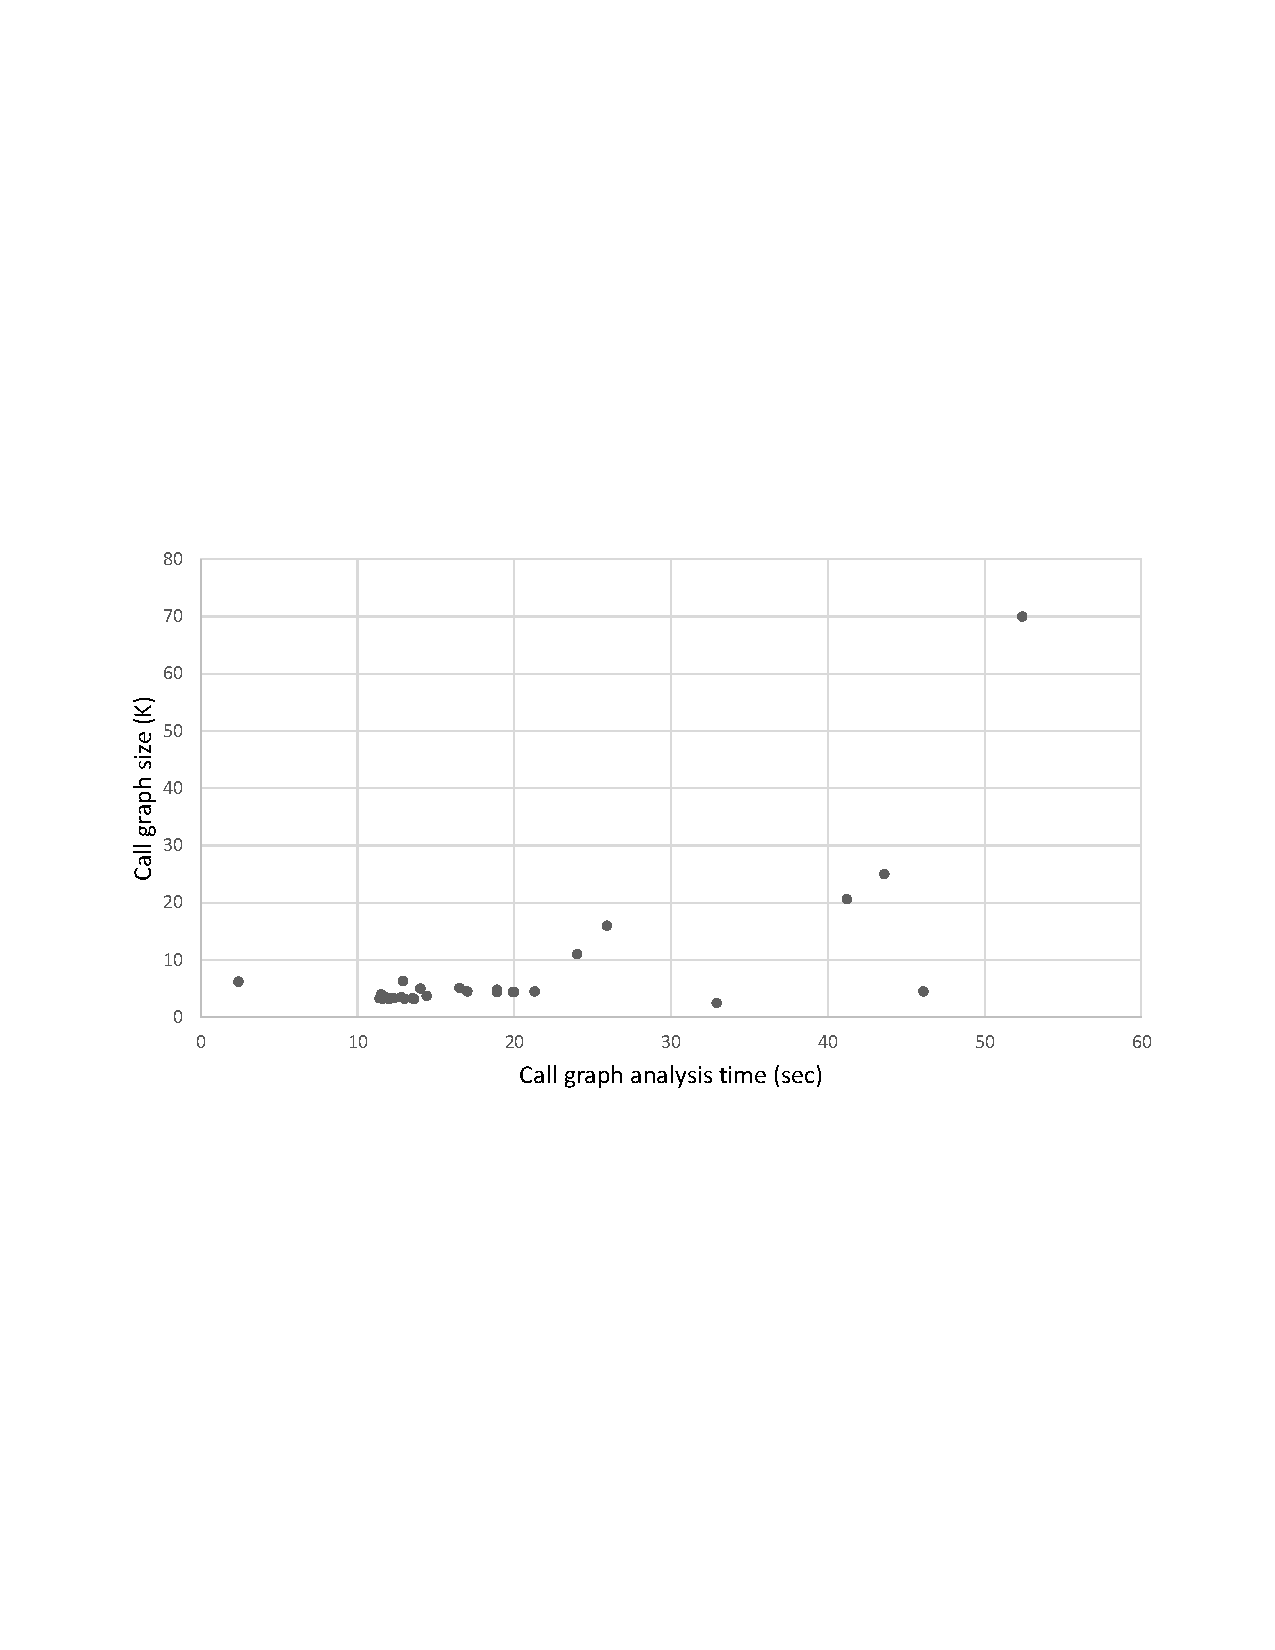
\includegraphics[scale = .35]{images/CgSizeVsTime.pdf}
\caption{Performance statistics of call graph size vs. time}
\label{fig:perf:callgraph}
\end{figure}


\begin{figure}[t]
\centering
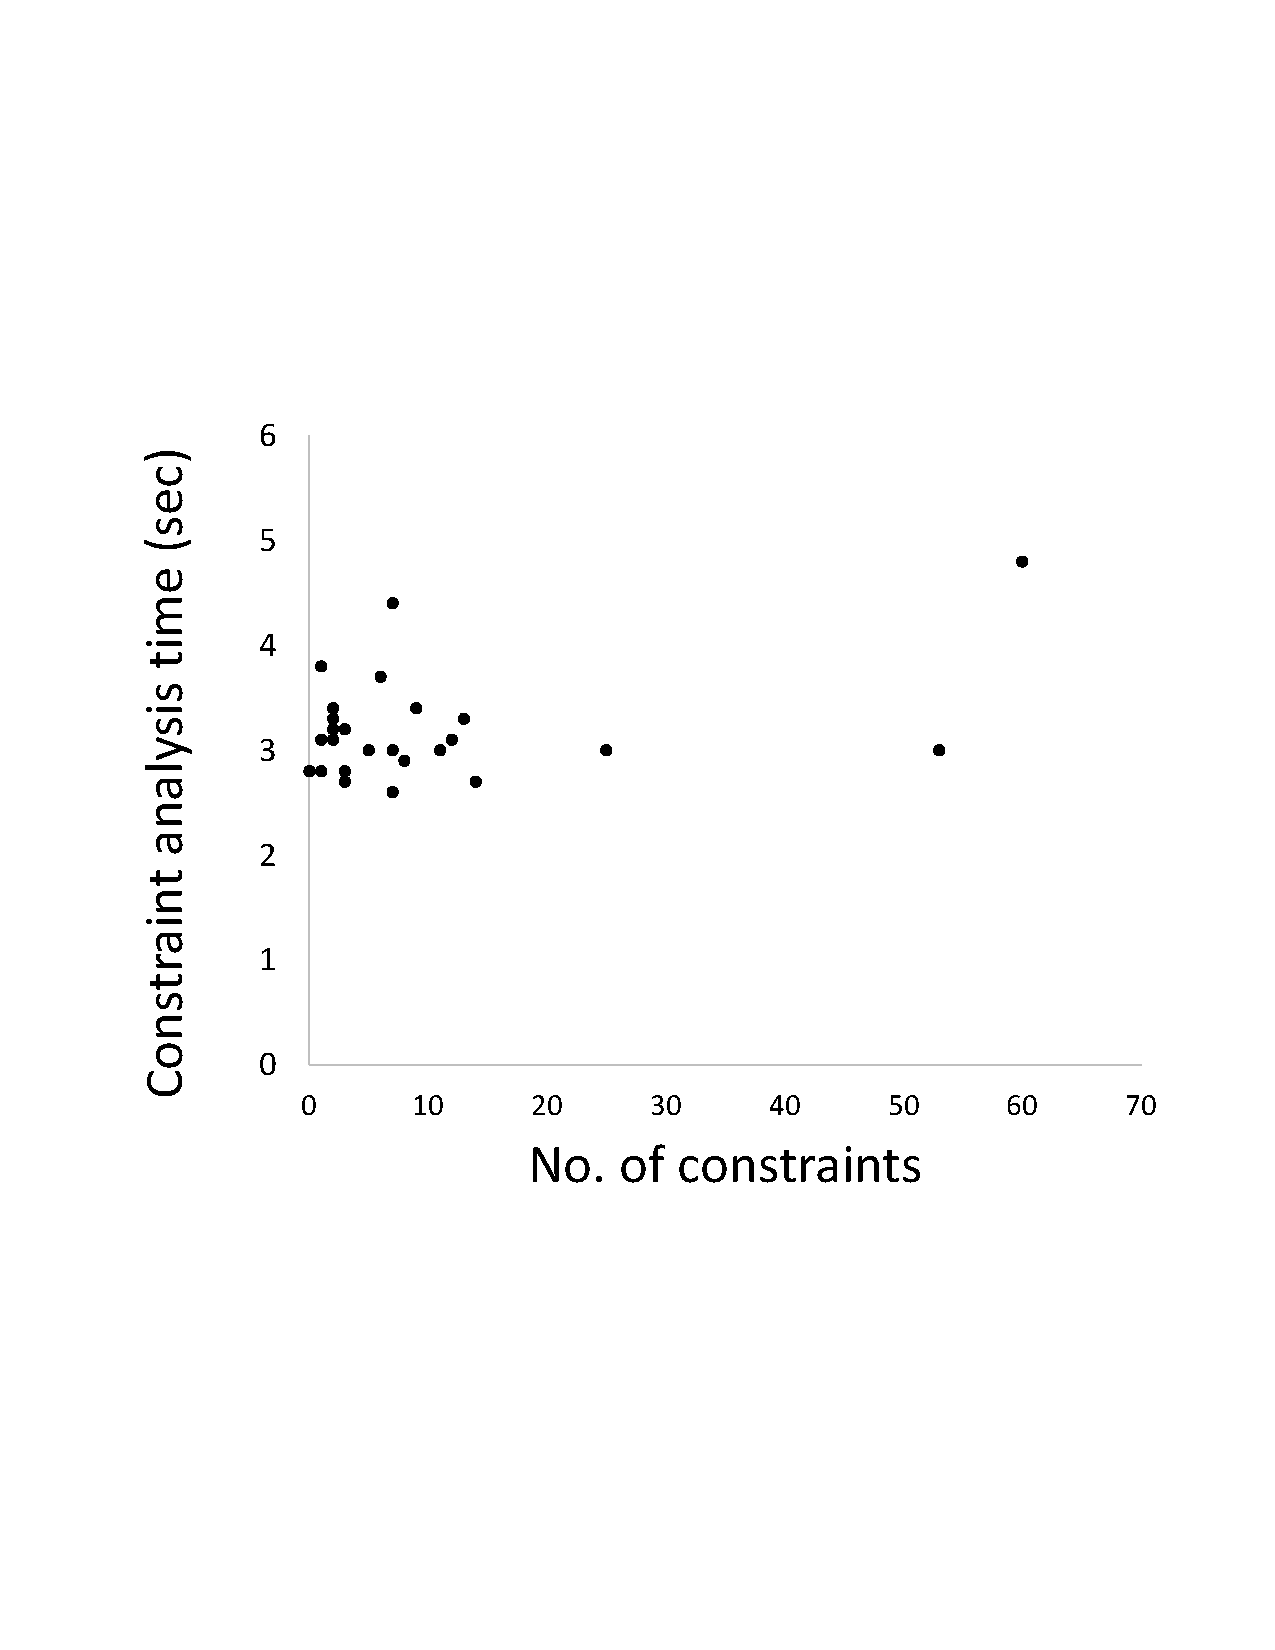
\includegraphics[scale = .35]{images/ConstraintsVsTime.pdf}
\caption{Performance statistics of constraint vs. time}
\label{fig:perf:constraints}
\end{figure}

\begin{figure}[t]
\centering
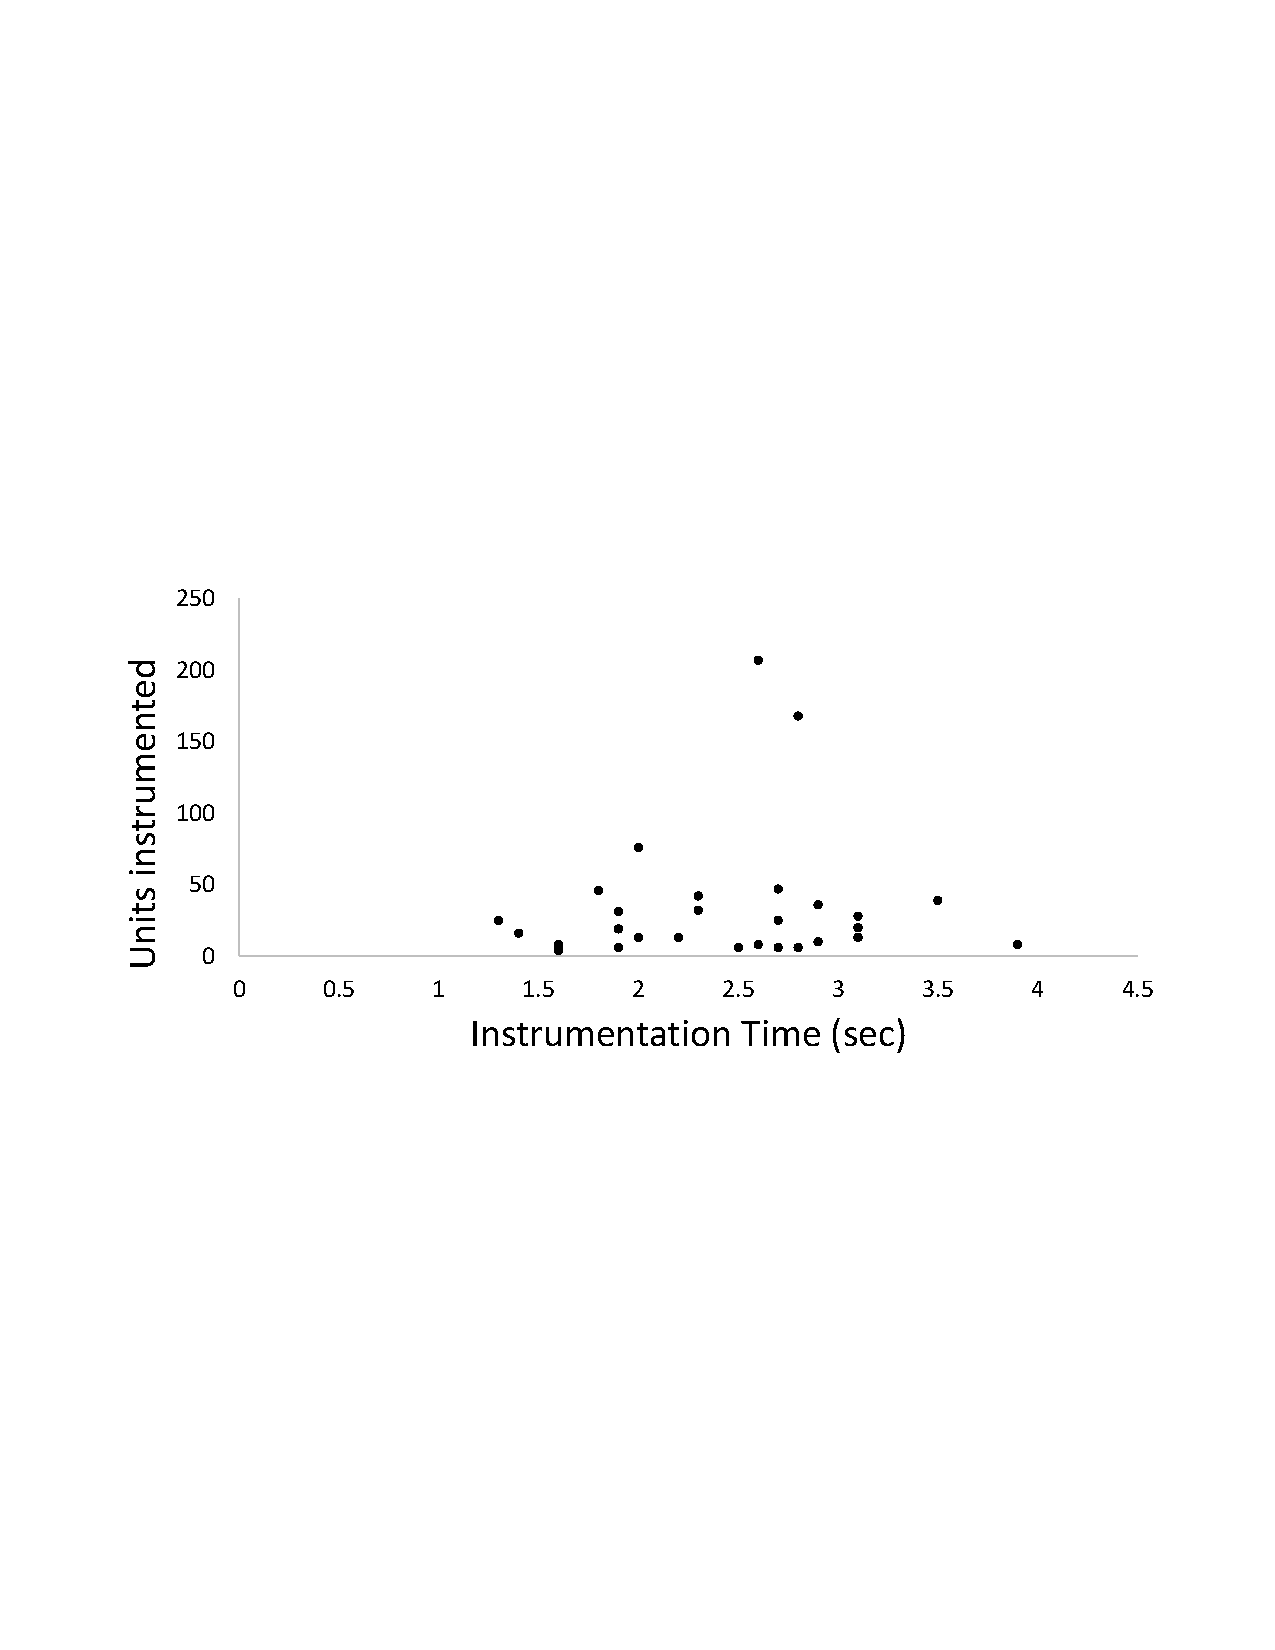
\includegraphics[scale = .35]{images/InstrumentationVsTime.pdf}
\caption{Performance statistics of instrumentation size vs time}
\label{fig:constraintHisto}
\end{figure}


%not required
% \begin{figure}
%         \centering
%         \begin{subfigure}[b]{0.3\textwidth}
%                 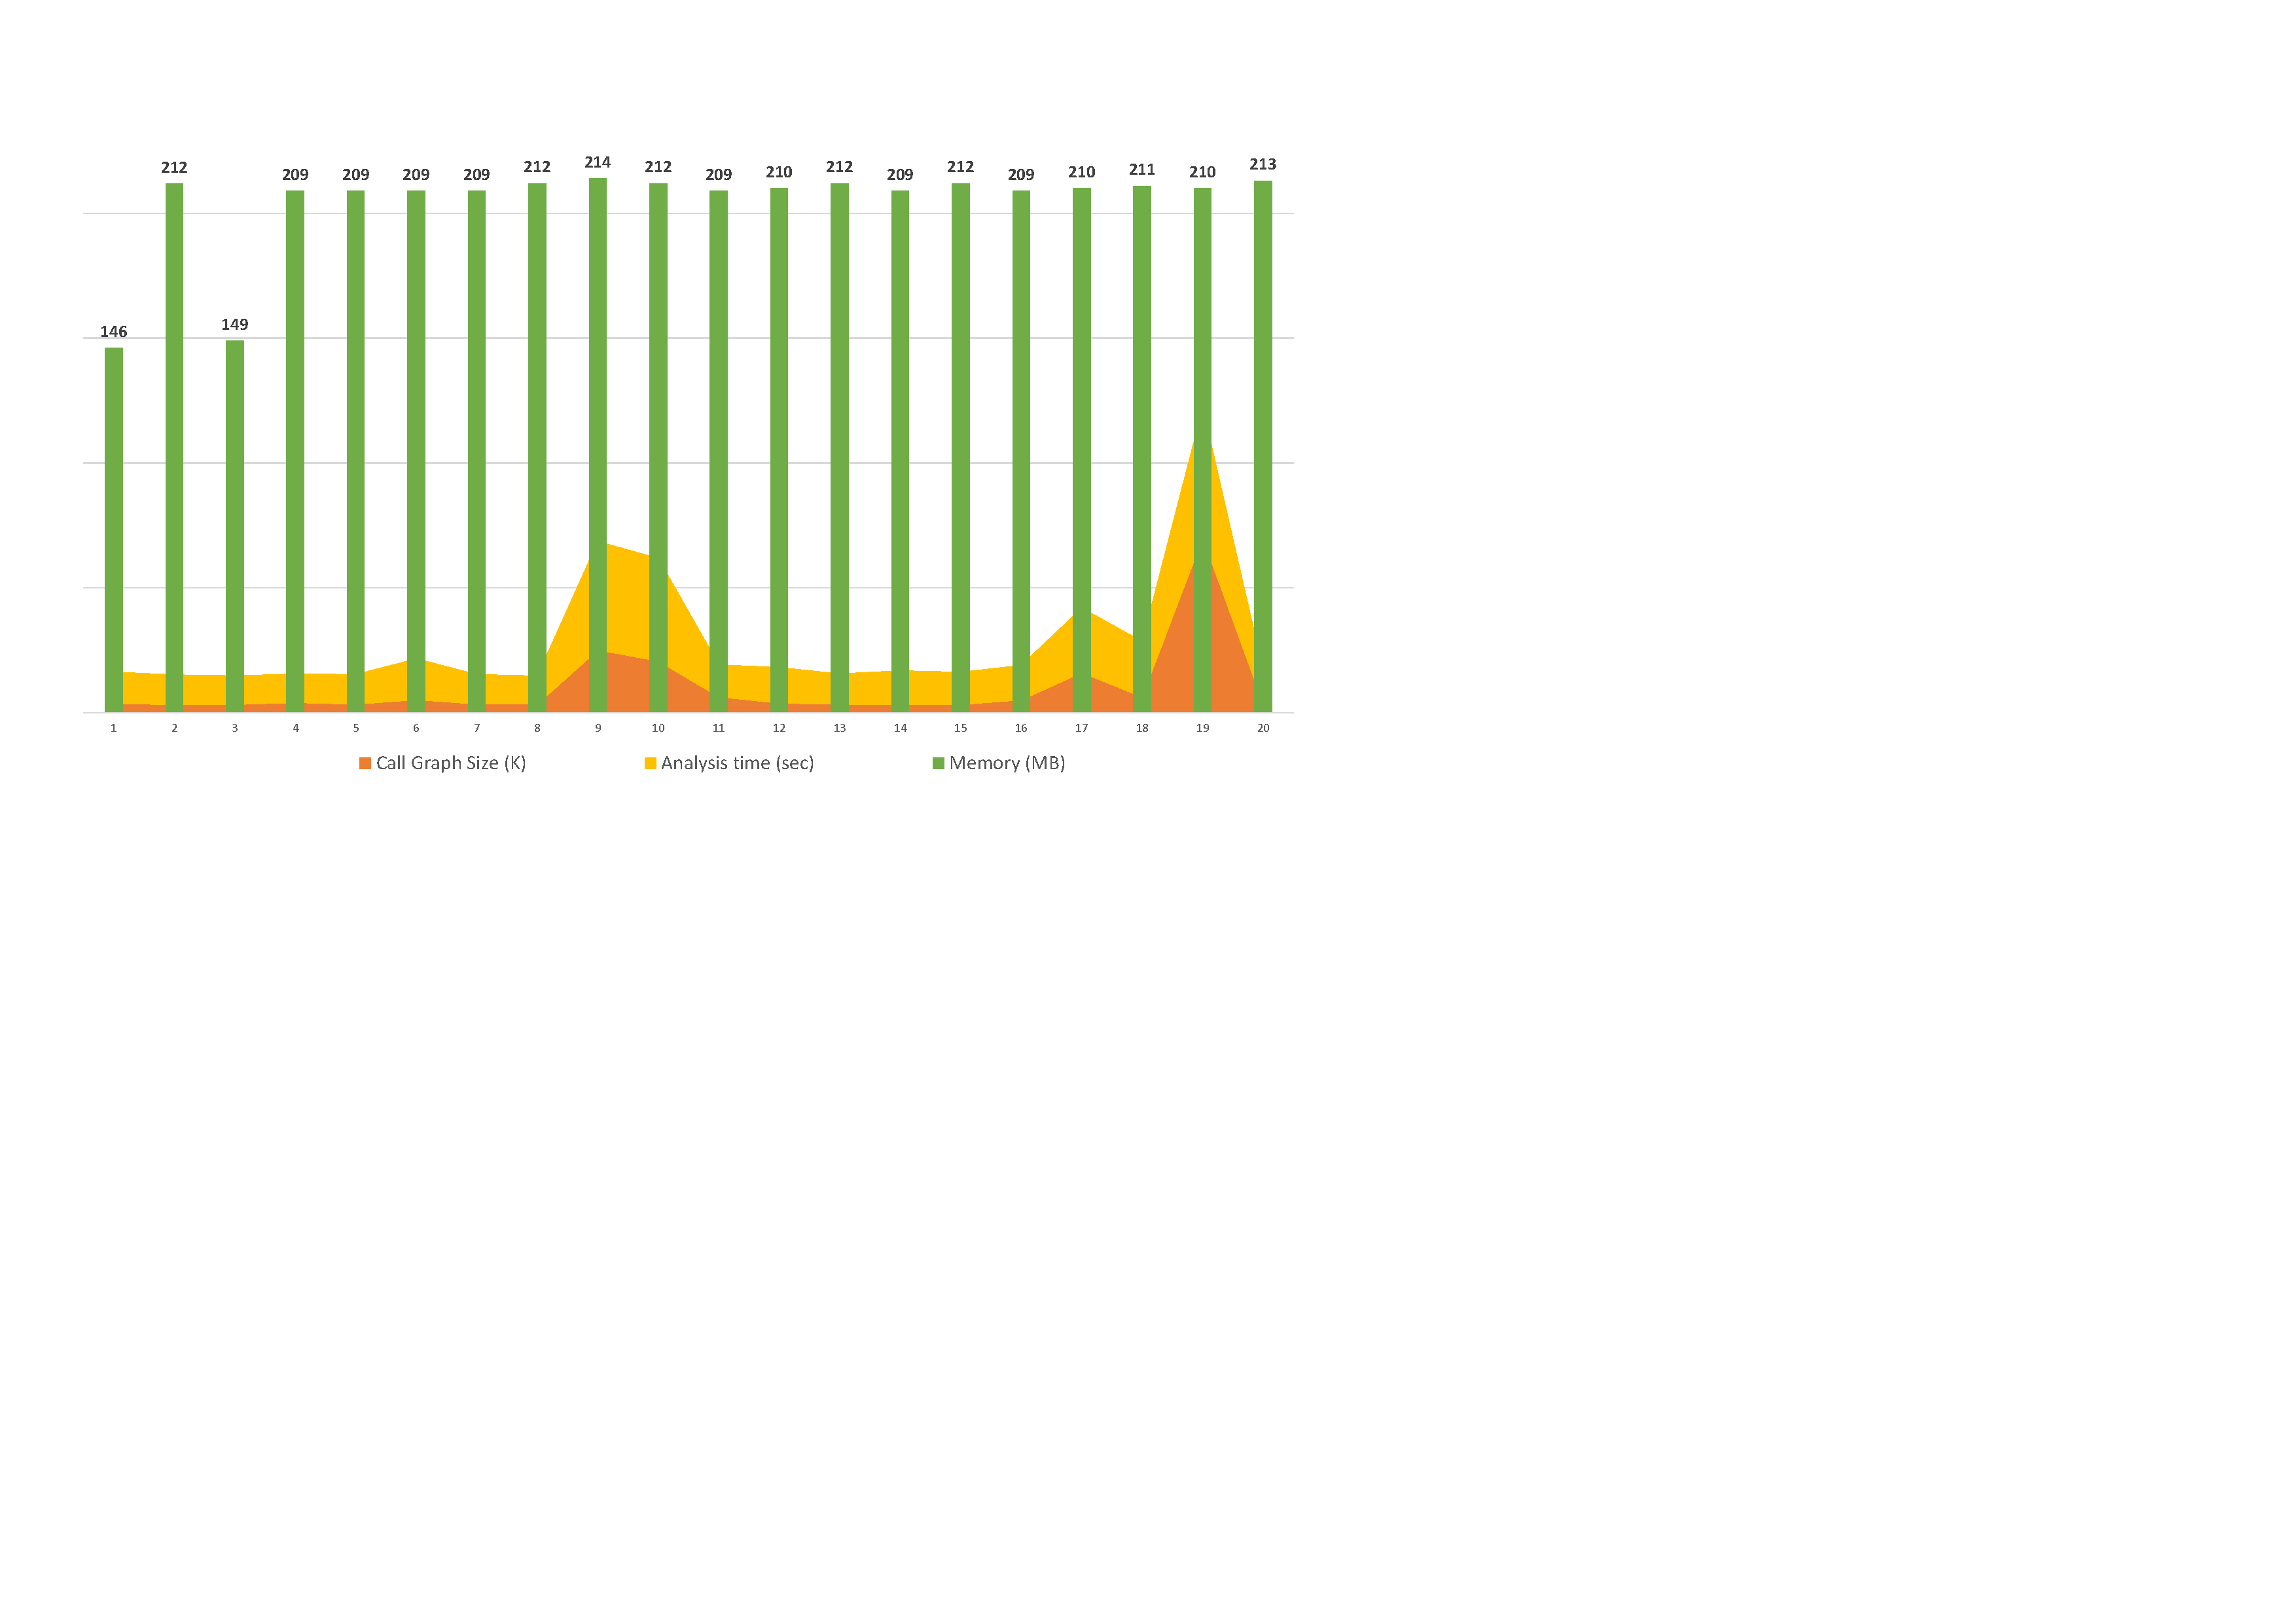
\includegraphics[width=\textwidth]{images/CallGraphHisto.pdf}
%                 \caption{A gull}
%                 \label{fig:gull}
%         \end{subfigure}%
%         ~ %add desired spacing between images, e. g. ~, \quad, \qquad, \hfill etc.
%           %(or a blank line to force the subfigure onto a new line)
%         \begin{subfigure}[b]{0.3\textwidth}
%                 \includegraphics[width=\textwidth]{tiger}
%                 \caption{A tiger}
%                 \label{fig:tiger}
%         \end{subfigure}
%         ~ %add desired spacing between images, e. g. ~, \quad, \qquad, \hfill etc.
%           %(or a blank line to force the subfigure onto a new line)
%         \begin{subfigure}[b]{0.3\textwidth}
%                 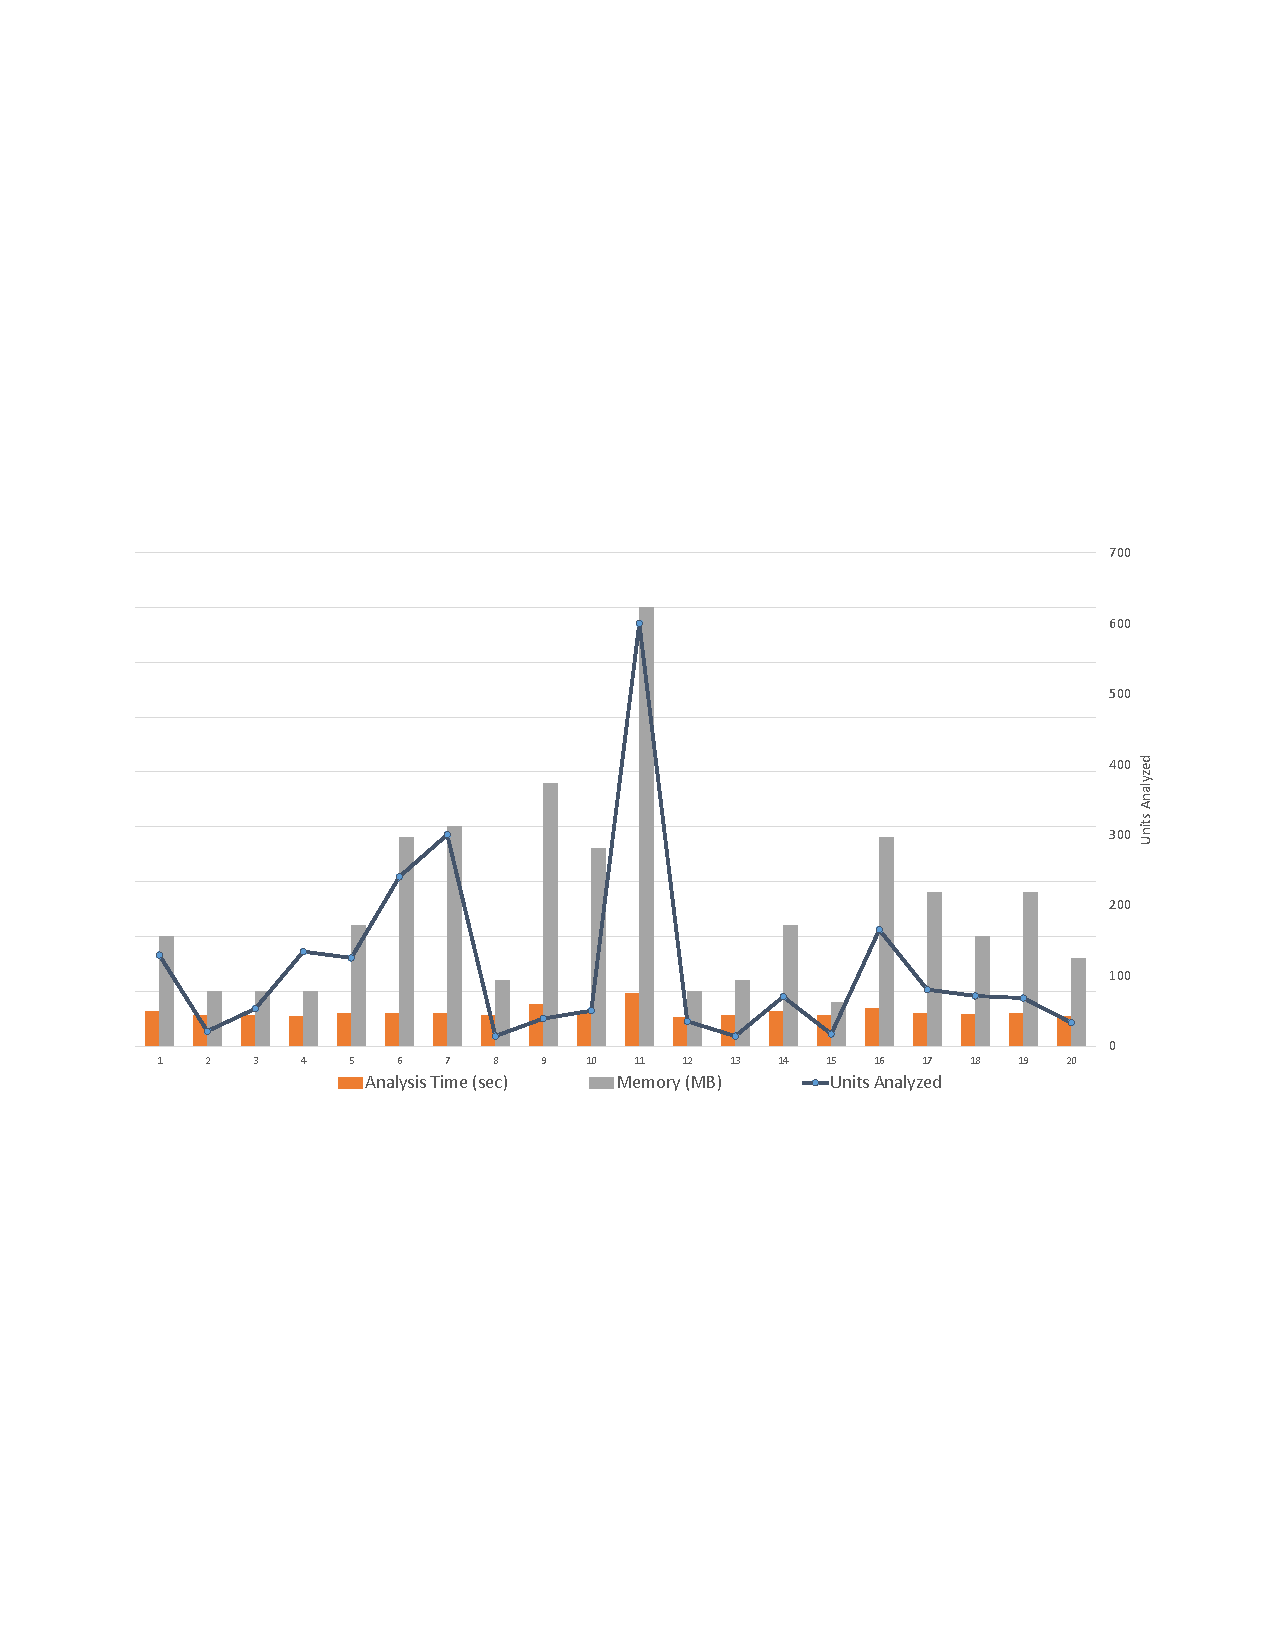
\includegraphics[width=\textwidth]{images/ConstraintHisto.pdf}
%                 \caption{A mouse}
%                 \label{fig:mouse}
%         \end{subfigure}
%         \caption{Pictures of animals}\label{fig:animals}
% \end{figure}
